\documentclass{beamer}
\usepackage[T1]{fontenc}
\usepackage[ngerman]{babel}
\usepackage[utf8]{inputenc}
\usepackage[babel,german=quotes]{csquotes}
\usepackage{amsmath,amsfonts,amssymb}
\usepackage{hyperref}
\usepackage{lmodern}

\usetheme{JuanLesPins}
\usepackage{beamerthemeshadow}

\usepackage[sort&compress,comma,super,square]{natbib}
%\bibliographystyle{apalike} % Or your specific bibliographystyle
\bibliographystyle{unsrtdin}
%\bibliographystyle{gerplain}


\title{cowbus -- a small home automation bus}
\author[R. Backhaus, K. Höllring, P. Kanzler, J. Schnurrer, M. Zapf]{Robin\,Backhaus \and Kevin\,Höllring \and Patrick\,Kanzler \and Josef\,Schnurrer \and Michael\,Zapf}
\date{28.01.2015}


\begin{document}
\frame{\titlepage}

\section{cowbus -- a small home automation bus}
\begin{frame}
    \frametitle{Ziele und Ideen}

    \begin{itemize}
        \item Mesh-Netzwerk
        \item dezentrale Organisation
        \item evtl. 6LoWPAN-basiert
        \item Gateway zu (vorhandenem) Ethernet \\
            (z.B. zur Nutzung mit \emph{OpenHAB})
    \end{itemize}

    \leavevmode
    \makebox(0,0){\put(220,0){
        \includegraphics[scale=0.3]{img/openhab-logo-square.png}
    }}
\end{frame}

\begin{frame}[plain]
    \center
    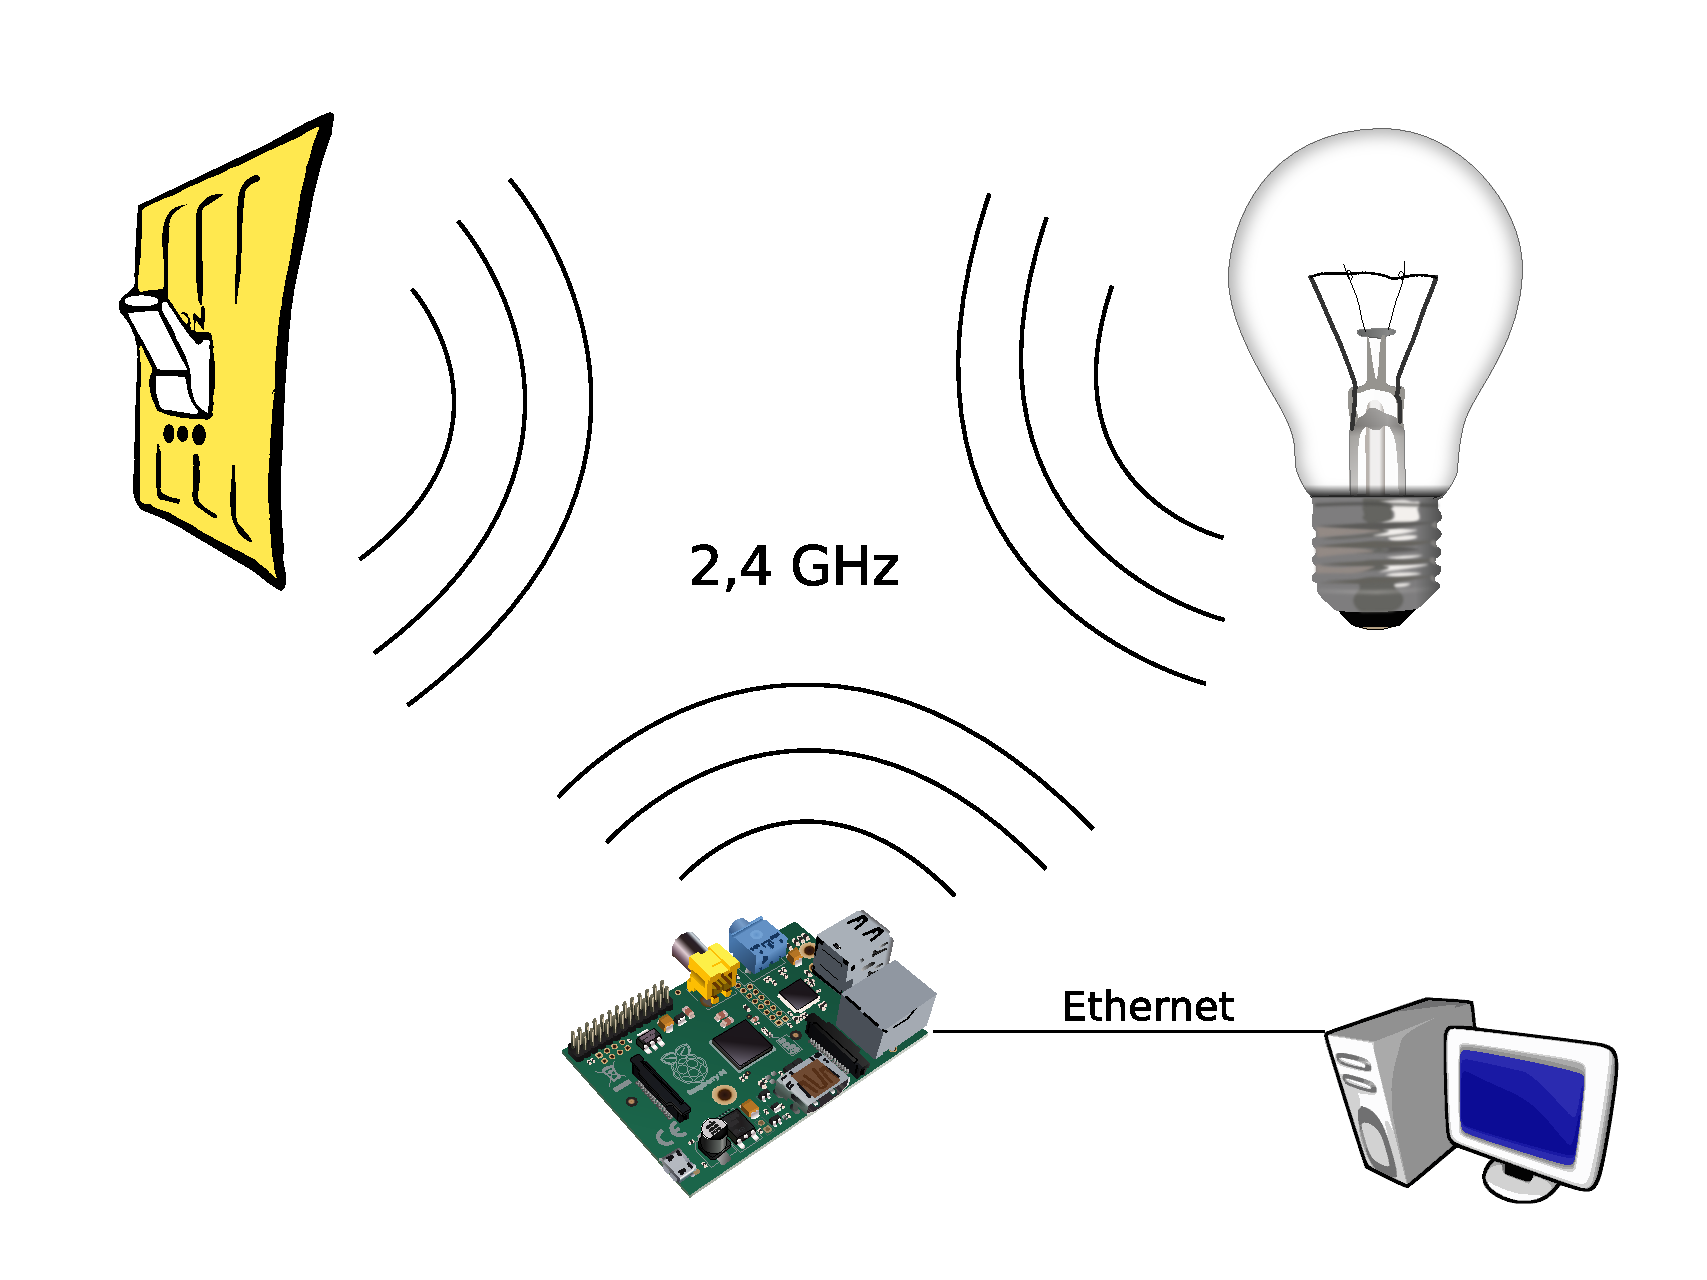
\includegraphics[scale=0.4]{img/system}
\end{frame}

\begin{frame}
    \frametitle{Hardware}

    \begin{itemize}
        \item \enquote{Prototyping-Board}
        \item Batterie-/Akkubetrieben (oder USB)
        \item ARM Cortex M0: STM32F030C8T6
            \begin{itemize}
                \item bis zu 48MHz
                \item Gehäuse: LQFP48 (7x7 mm)
            \end{itemize}
        \item RGB-LED und normale LED, 3 Taster
    \end{itemize}
\end{frame}

\begin{frame}
    \frametitle{Firmware}

    \begin{itemize}
        \item basiert auf RIOT OS (\url{http://www.riot-os.org/})
            \begin{itemize}
                \item \enquote{The friendly Operating System for the Internet of Things.}
                \item Multithreading
                \item gut portierbar (Schichtenarchitektur)
                \item Lizenz: LGPLv2
            \end{itemize}
    \end{itemize}

    \leavevmode
    \makebox(0,0){\put(200,-80){
        \includegraphics[width=0.4\linewidth]{img/logo-large.png}
    }}
\end{frame}

\begin{frame}
    \frametitle{Gateway}

    \begin{itemize}
        \item Kommunikation mit IP-Netzen
        \item erste Variante: Raspberry Pi mit Funkmodul
            \begin{itemize}
                \item Selbst Knoten im Funknetz
                \item Übersetzt Nachrichten: IP $\Leftrightarrow$ Funk
                \item HTML-Client mit Websockets
            \end{itemize}
    \end{itemize}
\end{frame}

%\begin{block}{Blocktitel}
%Blocktext
%\end{block}
%
%\begin{exampleblock}{Blocktitel}
%Blocktext
%\end{exampleblock}
%
%
%\begin{alertblock}{Blocktitel}
%Blocktext
%\end{alertblock}
%}

\nocite*
\bibliography{2015-01-28_cowbus}{}

\end{document}

